\chapter{Textos}

Neste capítulo nós veremos os elementos HTML textuais básicos. Além de aprender a usar vários tipos de elementos textuais básicos, vamos também conhecer o significado que cada tipo de elemento HTML carrega com ele, o que também é conhecido como \textbf{semântica} do elemento.

Existem elementos HTML específicos para títulos, parágrafos, códigos-fontes, citações, links e outras finalidades. Apesar disso, é possível (mas não recomendado) usar um elemento de parágrafo desempenhando o papel de um título, por exemplo, no que diz respeito ao visual. O problema é que o significado desse conteúdo não estará coerente, porque você estará mostrando um título em um elemento que deveria mostrar o texto de um parágrafo. 

Esse tipo de incoerência pode impedir que um site seja compreendido e indexado corretamente por ferramentas de busca e pode impactar negativamente na acessibilidade de uma página. Portanto, é importante que se utilize os elementos HTML para os propósitos definidos por seus significados.

Como mencionei, essa questão está relacionada com a semântica dos elementos. Sempre que ouvir o termo \textbf{semântica}, lembre-se de que isso diz respeito ao significado transmitido por cada tipo de elemento HTML. Visto isso, vamos começar a estudar os elementos básicos da HTML para exibição de conteúdo textual.

\section{Títulos e Subtítulos}

Vamos começar pelos elementos responsáveis pela adição de títulos e subtítulos em uma página. Os elementos são o \var{h1}, \var{h2}, \var{h3}, \var{h4}, \var{h5} e \var{h6}. Quanto à semântica, todos esses elementos correspondem a títulos, mas os de nível menor são mais importantes do que os títulos de nível maior. Portanto, quanto maior o nível, menor sua importância semântica.

Nós vamos iniciar o estudo sobre o código dos elementos textuais básicos criando um documento HTML correspondente a um artigo fictício, contendo apenas alguns títulos e parágrafos e, posteriormente, vamos incrementar esse documento com outros elementos. O exemplo \ref{code:texto_basico} mostra o código inicial desse documento HTML.

\begin{htmlcode}{Elementos textuais básicos.}{code:texto_basico}
<!DOCTYPE>
<html lang="pt-br">
<head>
    <meta charset="UTF-8">
    <meta name="viewport" content="width=device-width, initial-scale=1.0">
    <title>Elementos Textuais Básicos</title>
</head>
<body>
    <h1 id="titulo">Elementos Textuais Básicos</h1>
    <hr>
    <p>Cupidatat do veniam reprehenderit cillum sunt. Est quis mollit incididunt
    voluptate incididunt eiusmod quis veniam. Non nulla officia voluptate.</p>
    <p>Et magna id sunt commodo ea. Non occaecat ex duis officia laborum pariatur
    proident laborum sit ullamco fugiat anim aliquip. Incididunt in amet ad.</p>
    <!-- Este é um comentário -->
    <p>Lorem velit laborum irure labore ad dolor aliquip minim elit laboris est.
    Ex Lorem consequat culpa pariatur esse id laboris ex aute est. Nostrud</p>
    <h2 id="subtitulo">Subtítulo Qualquer</h2>
    <p>Cupidatat do veniam reprehenderit cillum sunt. Est quis mollit incididunt
    voluptate incididunt eiusmod quis veniam. Non nulla officia voluptate.</p>
</body>
</html>
\end{htmlcode}

Este código HTML do exemplo \ref{code:texto_basico} corresponde a uma página web bem simples. Na linha 1, o elemento \var{<!DOCTYPE>} indica o tipo de documento que está sendo usado. O valor vazio (sem atributos) indica que este é um documento HTML5, que é a última versão da HTML. Na linha 2, o elemento \var{<html lang="pt-br"\textgreater} é o elemento raiz de todo o documento HTML. O atributo \var{lang} especifica o idioma da página, que, neste caso, é o Português do Brasil. Na linha 3, o elemento \var{<head>} contém informações sobre a página, como o título da página e o tipo de codificação de caracteres. Na linha 4, o elemento \var{<meta charset="UTF-8"\textgreater} especifica o tipo de codificação de caracteres que está sendo usado na página. ``UTF-8'' é uma codificação de caracteres amplamente utilizada e suportada que permite a exibição de caracteres de diferentes idiomas. A linha 5 apresenta o elemento \var{<meta name="viewport"\space content="width=device-width, initial-scale=1.0"\textgreater}, que controla como a página é exibida em dispositivos móveis. A largura da página será igual à largura do dispositivo e a escala inicial será igual a 1.0. Na linha 6, o elemento \var{<title>} define o título da página, que é exibido na guia do navegador.

Entre as linhas 8 e 21 estão os elementos de conteúdo da página, iniciado pelo elemento \var{<body>}. Na linha 9, o elemento \var{<h1 id="titulo"\textgreater Elementos Textuais Básicos</h1>} é um elemento de cabeçalho de nível 1 que fornece um título para a página. O atributo \var{id} fornece um nome único para este elemento, que pode ser usado para referenciar este elemento em outros lugares na página, principalmente em links e códigos Javascript. Na linha 10, o elemento \var{<hr>} cria uma linha horizontal na página. Nas linhas 11, 13, 16 e 19 temos elementos \var{<p>}, que representam um parágrafo de texto. O código da linha 15, \var{<!-- Este é um comentário -->}, é um comentário HTML, ou seja, um texto que não será exibido na página. Comentários são usados para adicionar notas ou informações úteis sobre algo presente no código-fonte para facilitar o entendimento de outra pessoa que leia este código. Na linha 18, o elemento \var{<h2 id="subtitulo"\textgreater Subtítulo Qualquer</h2>} é outro elemento de cabeçalho, porém, de nível 2, que fornece um subtítulo para a página. Ele é menos relevante e visualmente menor que o \var{h1} e é usado para se criar seções secundárias no documento. A figura \ref{fig:rend_html_basico} mostra o documento HTML do exemplo \ref{code:texto_basico} renderizado.

\begin{figure}[ht!]
    \centering
    \frame{
    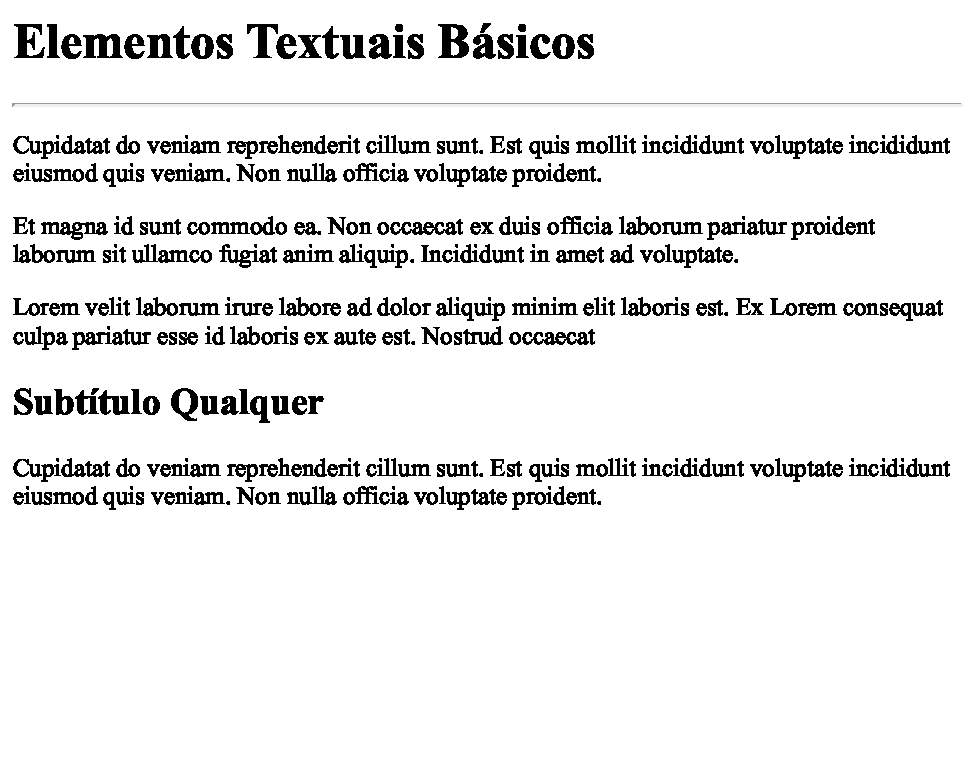
\includegraphics[width=1\textwidth, trim={0 4cm 0 0}]{Images/chapter03/html_basico1.pdf}}
    \caption{Renderização do código HTML do exemplo \ref{code:texto_basico}.}
    \label{fig:rend_html_basico}
\end{figure}

\section{Parágrafos e Quebras}

O elemento \var{<p>} é usado para definir um parágrafo em uma página HTML. O elemento \var{<p>} é um elemento de bloco e é usado para agrupar um bloco de texto em um único parágrafo. Elementos de bloco são aqueles que ocupam um bloco horizontal inteiro, não admitindo vizinhos laterais. O elemento \var{<p>} é importante porque ajuda a organizar e estruturar o conteúdo de uma página HTML. Ao usar o elemento \var{<p>}, você pode separar diferentes ideias e pensamentos em parágrafos individuais, o que torna o texto mais fácil de ler e entender. 

Por padrão, espaços, tabulações e as quebras de linha inseridas pelo pressionamento da tecla \textit{Enter} \textbf{são condensados em um único caractere de espaço} durante a renderização da página. Esse comportamento ocorre em qualquer conteúdo presente em um elemento HTML, exceto no elemento \var{<pre>}, apresentado mais adiante. Contudo, se você quiser forçar uma quebra de linha, você pode usar um elemento \var{<br>}. O elemento \var{<hr>} também insere uma quebra, porém, adiciona uma linha horizontal dividindo o conteúdo em duas partes. O elemento \var{<hr>} pode ser interessante para se criar separação de seções em um documento. O código \ref{code:p_br_hr} apresenta um exemplo de uso de parágrafos e quebras e a figura \ref{fig:p_br_hr} mostra a renderização desse código.

\begin{htmlcode}{Elementos textuais básicos.}{code:p_br_hr}
<p>Este é um parágrafo que contém algum texto. Aqui está uma quebra de linha:<br>
Este é outro texto que aparece em uma nova linha. Aqui está outra quebra de linha:
<br><br> Este é outro texto que aparece duas linhas abaixo. O elemento &lt;hr&gt;
pode ser usado para adicionar uma linha horizontal:</p>
<hr>
<p>Este é outro parágrafo que contém algum texto. Aqui está outra quebra de linha:
<br> Este é outro texto que aparece em uma nova linha. Aqui está outra quebra de
linha: <br><br> Este é outro texto que aparece duas linhas abaixo.</p>
\end{htmlcode}

\begin{figure}[ht!]
    \centering
    \frame{
    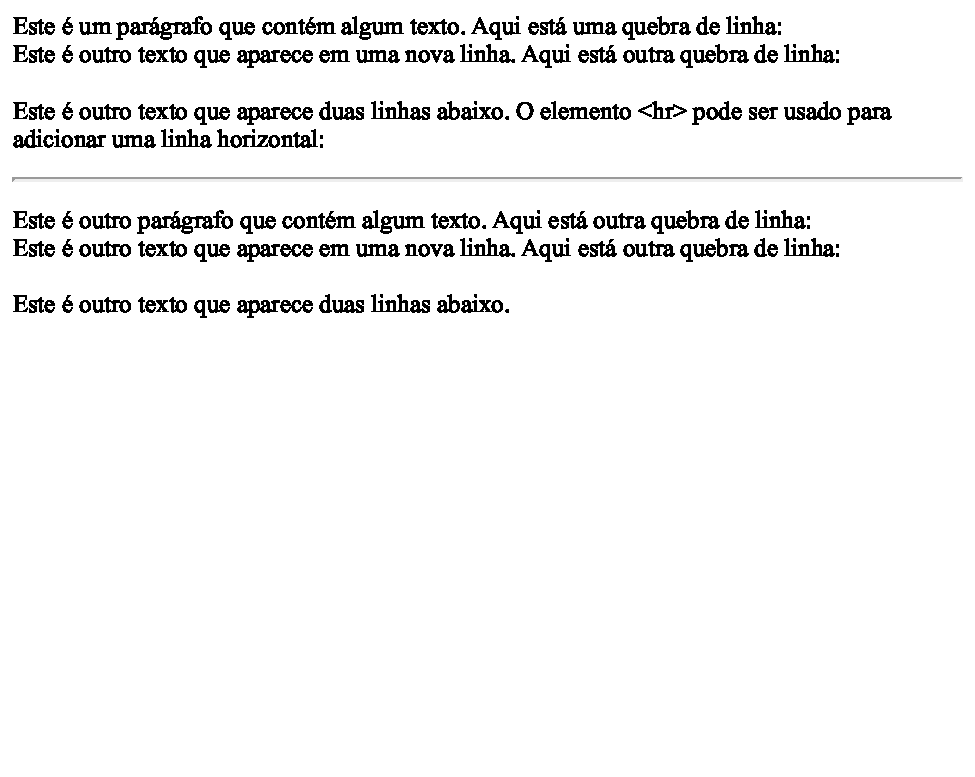
\includegraphics[width=1\textwidth, trim={0 7.5cm 0 0}]{Images/chapter03/html_p_br_hr.pdf}}
    \caption{Renderização do código HTML do exemplo \ref{code:p_br_hr}.}
    \label{fig:p_br_hr}
\end{figure}

\section{Texto Pré-Formatado}

O elemento \var{<pre>} é usado em HTML para apresentar texto pré-formatado. Quando você usa o elemento \var{<pre>}, o navegador preserva a formatação original do texto, incluindo espaços em branco, quebras de linha e tabulações. Isso é útil quando você precisa apresentar texto que precisa ser exibido exatamente como está no código-fonte, sem ajustes automáticos de formatação. Além disso, por padrão, o elemento \var{<pre>} usa fonte monoespaçada, que são aquelas fontes em que todos os caracteres ocupam a mesma largura em pixels, como a fonte ``Courier New''. O exemplo \ref{code:pre} mostra o código de um exemplo de texto pré-formatado usando o elemento \var{<pre>}, enquanto a figura \ref{fig:pre} mostra a renderização desse exemplo.

\begin{htmlcode}{Texto Pré-Formatado.}{code:pre}
<pre>
Este é um exemplo de texto
   pré-formatado. Note como
   os espaços em branco e as
   quebras de linha são preservados.
</pre>
\end{htmlcode}

\begin{figure}[htpb!]    
    \frame{
    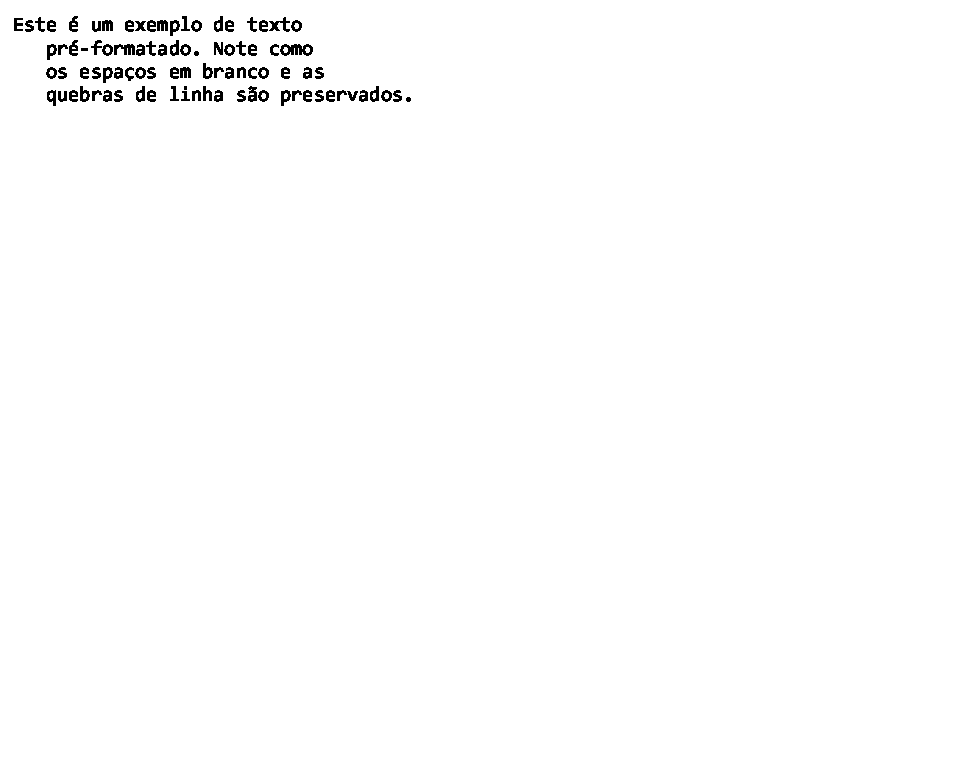
\includegraphics[width=.5\textwidth, trim={0 11cm 8cm 0}]{Images/chapter03/html_pre.pdf}}
    \caption{Renderização do texto pré-formatado do exemplo \ref{code:pre}.}
    \label{fig:pre}
\end{figure}

\section{Texto de Código-Fonte}

O elemento \var{<code>} é usado em HTML para indicar um bloco de código ou texto que representa um comando, uma função ou outra representação de código-fonte. O navegador geralmente apresenta o texto dentro do elemento \var{<code>} em uma fonte monoespaçada, para destacá-lo como código. O exemplo \ref{code:code} mostra o código HTML de um exemplo de texto de código-fonte usando o elemento \var{<code>} e a figura \ref{fig:code} mostra a renderização do exemplo.

\begin{htmlcode}{Texto de Código-Fonte.}{code:code}
<p>Você pode usar o seguinte código em JavaScript para exibir uma mensagem:</p>
<code>
  alert("Olá, mundo!");
</code>
\end{htmlcode}

\begin{figure}[ht!]    
    \frame{
    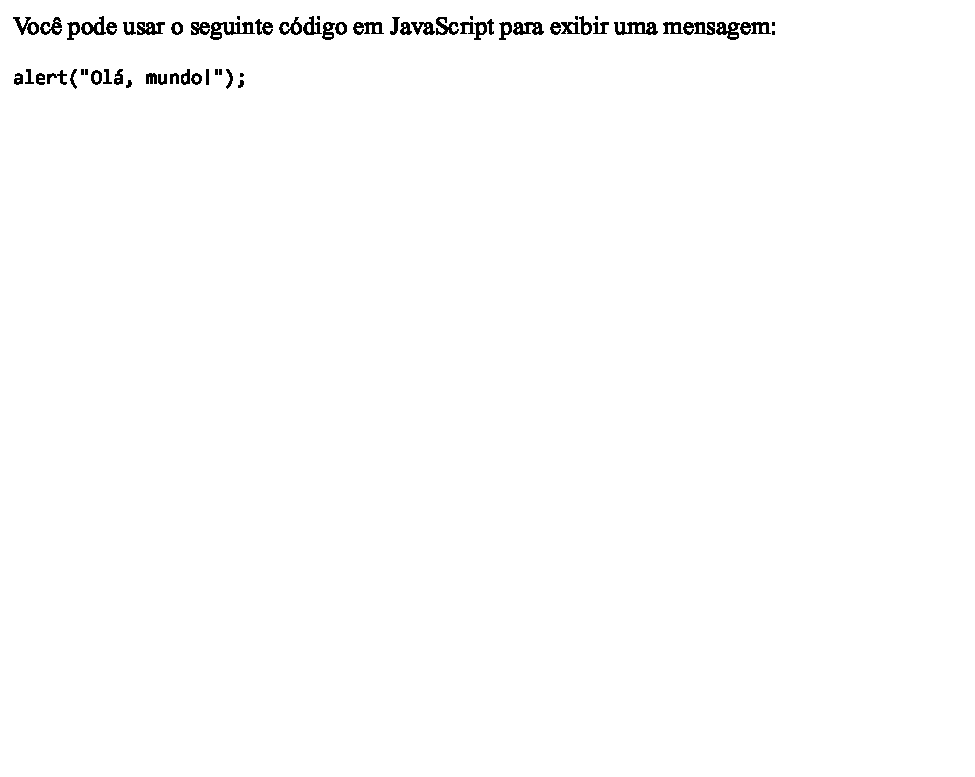
\includegraphics[width=.8\textwidth, trim={0 11cm 3cm 0}]{Images/chapter03/html_code.pdf}}
    \caption{Renderização do texto de código-fonte do exemplo \ref{code:code}.}
    \label{fig:code}
\end{figure}

A importância do elemento \var{<code>} é que ele permite que o autor da página identifique claramente um texto como código-fonte, o que ajuda a melhorar a legibilidade e acessibilidade do conteúdo. Além disso, ele permite que o navegador apresente o texto de forma diferenciada, o que pode ser útil para destacar o código em relação ao texto normal na página. É possível usar o elemento \var{<code>} em combinação com outros elementos, como o \var{<pre>}, para facilitar a organização do código com suas indentações.

\section{Links}

O elemento <a> é usado em HTML para criar links, permitindo que o usuário navegue para outras páginas do próprio site, para outros recursos na web ou para elementos da própria página. É um dos elementos mais importantes e amplamente usados em HTML. Portanto, existem três tipos principais de links que você pode criar com o elemento \var{<a>} em HTML: links internos, links externos e links ancorados.

\textbf{Links internos} são links que apontam para outras páginas do mesmo site. Por exemplo, se você tem um site com uma página inicial e uma página de contato, pode criar um link na página inicial que leva o usuário para a página de contato. Para criar um link interno, você especifica o caminho relativo da página de destino no atributo \var{href}. O código \ref{code:link_interno} mostra um exemplo de link interno que aponta para uma página do próprio site chamada ``contato.html''. 

\begin{htmlcode}{Link para interno apontando para uma página do próprio site.}{code:link_interno}
<p>Visite a <a href="contato.html">página de contato</a> para mais informações.</p>
\end{htmlcode}

\textbf{Links externos} são links que apontam para recursos fora do seu site. Por exemplo, você pode criar um link que leva o usuário para o site do Google. Para criar um link externo, você especifica o endereço completo da página de destino no atributo \var{href}. O código \ref{code:link_externo} mostra um exemplo de link externo que aponta para a página inicial do Google. Observe que o endereço completo do destino é passado, incluindo o nome de domínio, enquanto no link interno passamos somente o nome do recurso buscado.

\begin{htmlcode}{Link externo apontando para a página do Google.}{code:link_externo}
<p>Visite o site do <a href="https://www.google.com">Google</a>
para mais informações.</p>
\end{htmlcode}

\textbf{Links ancorados} são links que apontam para elementos dentro da própria página. Por exemplo, você pode ter um link na parte inferior da página que leva o usuário para uma seção específica na parte superior da página. Para criar um link ancorado, você especifica o identificador (atributo \var{id}) do elemento de destino no atributo \var{href} com o prefixo ``\#''. O código \ref{code:link_ancorado} mostra um exemplo de link ancorado que aponta para um elemento da própria página cujo identificador é ``secao1''.

\begin{htmlcode}{Link ancorado apontando para um elemento da própria página.}{code:link_ancorado}
<h2 id="secao1">Seção 1</h2>
...
<p>Volte para a <a href="#secao1">seção 1</a> para mais informações.</p>
\end{htmlcode}

Os links internos, externos e ancorados são importantes porque permitem que o usuário navegue facilmente pelo seu site e pela web, conectando páginas e recursos. Além disso, eles são uma ótima maneira de tornar o conteúdo da página acessível para usuários com necessidades especiais, como usuários de leitor de tela. A figura \ref{fig:links} mostra a renderização dos links dos exemplos anteriores.

\begin{figure}[ht!]    
    \frame{
    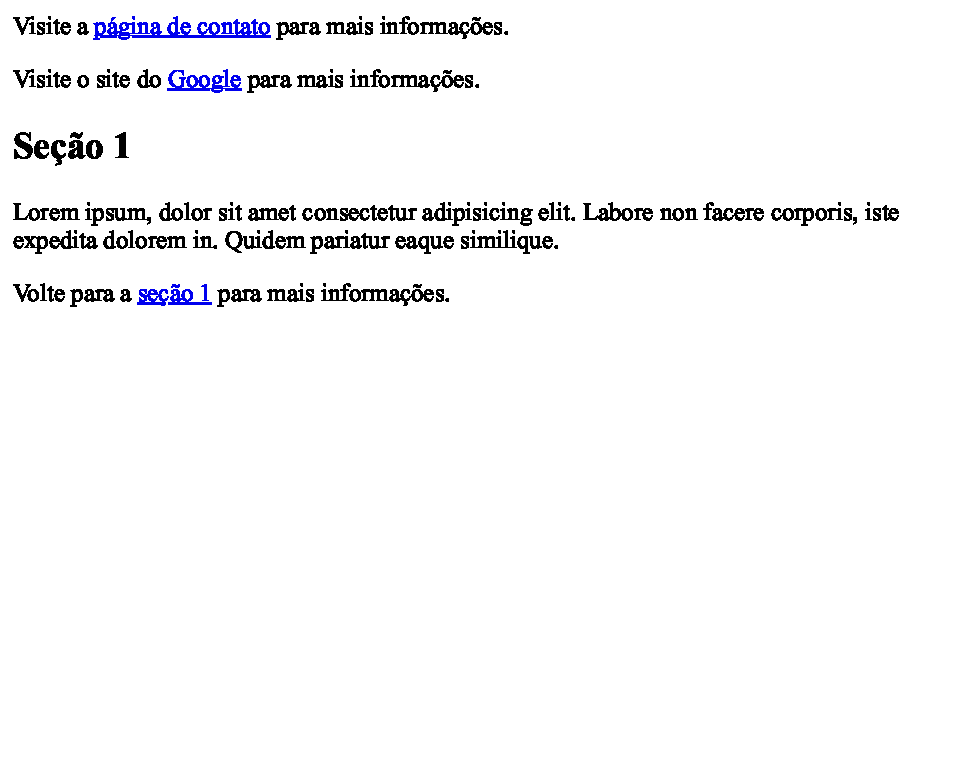
\includegraphics[width=1\textwidth, trim={0 7cm 0cm 0}]{Images/chapter03/html_links.pdf}}
    \caption{Renderização dos links dos exemplos desta seção.}
    \label{fig:links}
\end{figure}

\subsection{Local de Abertura do Link}

O atributo \var{target} é utilizado no elemento \var{<a>} para definir o local onde o recurso vinculado ao link deve ser aberto. Este atributo é útil, por exemplo, quando se deseja que um link seja aberto em uma janela ou guia diferente do navegador em que a página original está sendo exibida. O valor do atributo \var{target} pode ser um dos seguintes:

\begin{itemize}
    \item \var{\_self}: este é o valor padrão e indica que o link deve ser aberto na mesma janela ou guia do navegador em que a página atual está sendo exibida;
    \item \var{\_blank}: este valor indica que o link deve ser aberto em uma nova janela ou guia do navegador;
    \item \var{\_parent}: este valor indica que o link deve ser aberto na janela pai da janela atual. Esse valor é útil quando você está usando \textit{frames} em sua página, algo pouco usual nos dias atuais;
    \item \var{\_top}: Este valor indica que o link deve ser aberto na janela principal do navegador, substituindo todas as outras janelas ou guias abertas.
\end{itemize}

O exemplo \ref{code:link_target} mostra como usar o atributo \var{target} para abrir um link em uma nova guia do navegador.

\begin{htmlcode}{Link com atributo \var{target} para definição de local de abertura.}{code:link_target}
<a href="https://www.exemplo.com" target="_blank">Exemplo.com</a>
\end{htmlcode}

É importante lembrar que, ao usar o atributo \var{target}, você pode estar criando uma experiência de usuário diferente do esperado, já que o usuário pode ficar confuso ao abrir várias guias ou janelas do navegador sem saber como voltar à página anterior. Por isso, é recomendável usar esse atributo com moderação e fornecer ao usuário a opção de escolher se deseja ou não abrir um link em uma nova guia ou janela do navegador. Além disso, é importante lembrar que o uso do atributo \var{target} pode afetar a acessibilidade da página, e a melhor prática é sempre criar links que sejam fáceis de usar para todos os usuários.

\section{Formatação de Texto \textit{Inline}}

Os elementos \textit{inline} são elementos de formatação de texto em HTML que afetam apenas o texto dentro deles, sem afetar o leiaute da página. Eles são chamados de \textit{inline} porque eles são exibidos na linha com o texto ao invés de criar um novo bloco. Alguns exemplos comuns de elementos \textit{inline} de formatação de texto incluem:

\begin{itemize}
    \item \var{<strong>}: destaca o texto como sendo importante e normalmente é exibido em negrito;
    \item \var{<em>}: indica que o texto tem alguma ênfase e normalmente é exibido como itálico;
    \item \var{<mark>}: destaca o texto como sendo relevante e normalmente é exibido com fundo amarelo;
    \item \var{<abbr>}: usado para abreviaturas, com opção de exibir o significado completo ao passar o mouse sobre ele usando o atributo \var{title};
    \item \var{<del>}: é usado para marcar um texto que tenha sido excluído em uma versão anterior do documento e normalmente aparece riscado;
    \item \var{<ins>}: é usado para marcar um texto que tenha sido incluído em uma versão anterior do documento e normalmente aparece sublinhado;
    \item \var{<sub>}: é usado para exibir texto em índice inferior, ou seja, um texto menor que o tamanho normal que aparece abaixo da linha de base do texto;
    \item \var{<sup>}: é usado para exibir texto em índice superior, ou seja, um texto menor que o tamanho normal que aparece acima da linha de base do texto;
    \item \var{<small>}: é usado para exibir texto em tamanho menor que o tamanho normal do texto;
\end{itemize}

O exemplo \ref{code:html_inline} mostra o código de alguns dos elementos \textit{inline} citados anteriormente e a figura \ref{fig:html_inline} mostra a renderização desse código.

\begin{htmlcode}{Elementos \textit{inline} para formatação de texto.}{code:html_inline}
<p>Este é um texto <strong>importante</strong></p>
<p>Este é um texto <em>com ênfase</em></p>
<p>Este é um texto <mark>marcado</mark>.</p>
<p>Este o significado de <abbr title="Hypertext Markup Language">HTML</abbr></p>
<p>Este é um texto <del>excluído</del>.</p>
<p>Este é um texto <ins>inserido</ins>.</p>
<p>Este é um texto<sub>subscrito</sub>.</p>
<p>Este é um texto<sup>superescrito</sup>.</p>
<p>Este é um texto <small>menor que o tamanho normal</small>.</p>
\end{htmlcode}

\begin{figure}[ht!]    
    \frame{
    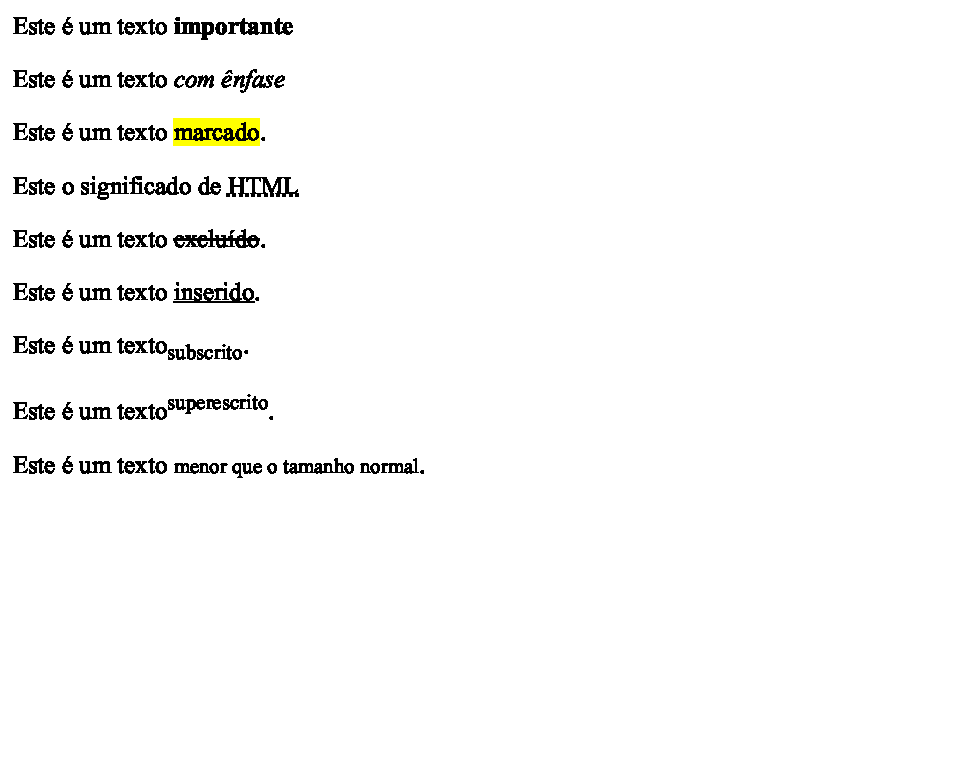
\includegraphics[width=1\textwidth, trim={0 4.7cm 3cm 0}]{Images/chapter03/html_inline.pdf}}
    \caption{Renderização dos elementos inline do código \ref{code:html_inline}.}
    \label{fig:html_inline}
\end{figure}

Os elementos inline de formatação de texto são importantes porque eles permitem que o autor da página destaque o texto de acordo com seu significado, melhorando a legibilidade e acessibilidade do conteúdo. Além disso, eles são uma ótima maneira de adicionar estilo e formatação ao texto sem afetar o layout da página.

Além dos elementos \textit{inline} mencionados anteriormente, há outros elementos \textit{inline} antigos em HTML que foram usados para formatação de texto, como \var{<b>}, \var{<i>}, \var{<s>}, \var{<u>}, \var{<big>} e outros, mas eles tornaram obsoletos. Portanto, estes elementos são menos recomendados do que os elementos \textit{inline} mencionados anteriormente, pois eles não têm um significado claro e acessível.

\section{Citações}

O elemento \var{<blockquote>} é usado para definir uma citação longa em um documento HTML, que, normalmente, são trechos de texto com mais de 3 linhas retirados de escritos de outros autores. Uma citação longa é um trecho de texto que é retirado de outro contexto e apresentado de forma destacada em um documento HTML. O elemento \var{<blockquote>} é útil para destacar citações importantes ou relevantes para o conteúdo da página. O exemplo \ref{code:html_blockquote} mostra o código de um texto que corresponde a uma citação.

\begin{htmlcode}{Bloco de citação longa.}{code:html_blockquote}
<blockquote cite="https://pt.wikipedia.org/wiki/Herbert_Kelleher">
  <p>O tempo é o melhor professor, o problema é que ele mata todos os seus alunos.</p>
  <footer>Herbert Kelleher</footer>
</blockquote>
\end{htmlcode}

Neste exemplo, o elemento \var{<blockquote>} é usado para marcar uma citação longa, que é o trecho ``O tempo é o melhor professor, o problema é que ele mata todos os seus alunos.''. O elemento \var{<footer}> é usado para fornecer informações sobre a fonte da citação, no caso, ``Herbert Kelleher''. Além disso, opcionalmente, é possível usar o atributo \var{cite} do elemento \var{<blockquote>} para fornecer uma URL que aponte para a fonte original da citação. Neste caso, a fonte original é uma página da Wikipédia.

Em resumo, o elemento \var{<blockquote>} é uma ferramenta poderosa para destacar citações importantes ou relevantes em um documento HTML. Ao usar o elemento \var{<blockquote>} e o atributo \var{cite}, você pode fornecer informações sobre a fonte da citação e tornar seu conteúdo mais confiável e acessível. 

O elemento \var{<blockquote>} resolve o problema das citações longas, mas temos também as citações curtas. As citações curtas são trechos de texto que são inseridos no meio de um parágrafo e não são destacados bloco. Para marcar citações curtas em HTML, você pode usar o elemento \var{<q>} e, opcionalmente, você também pode passar o atributo \var{cite} contendo a fonte da citação.

\begin{htmlcode}{Trecho de citação curta.}{code:html_quote}
<p>O filósofo Jean-Paul Sartre afirmou que 
    <q cite="https://pt.wikipedia.org/wiki/Jean-Paul_Sartre">
    O existencialismo é um humanismo</q>.</p>
\end{htmlcode}

Em resumo, o elemento \var{<q>} e o atributo \var{cite} são ferramentas úteis para marcar citações curtas em HTML. Assim como ocorre com a citação longa, ao usar esses recursos, você pode destacar o texto de uma citação curta, fornecer informações sobre a fonte da citação e tornar seu conteúdo mais claro e fácil de entender. A figura \ref{fig:html_citacoes} mostra os exemplos desta seção renderizados em uma página web.

\begin{figure}[ht!]    
    \frame{
    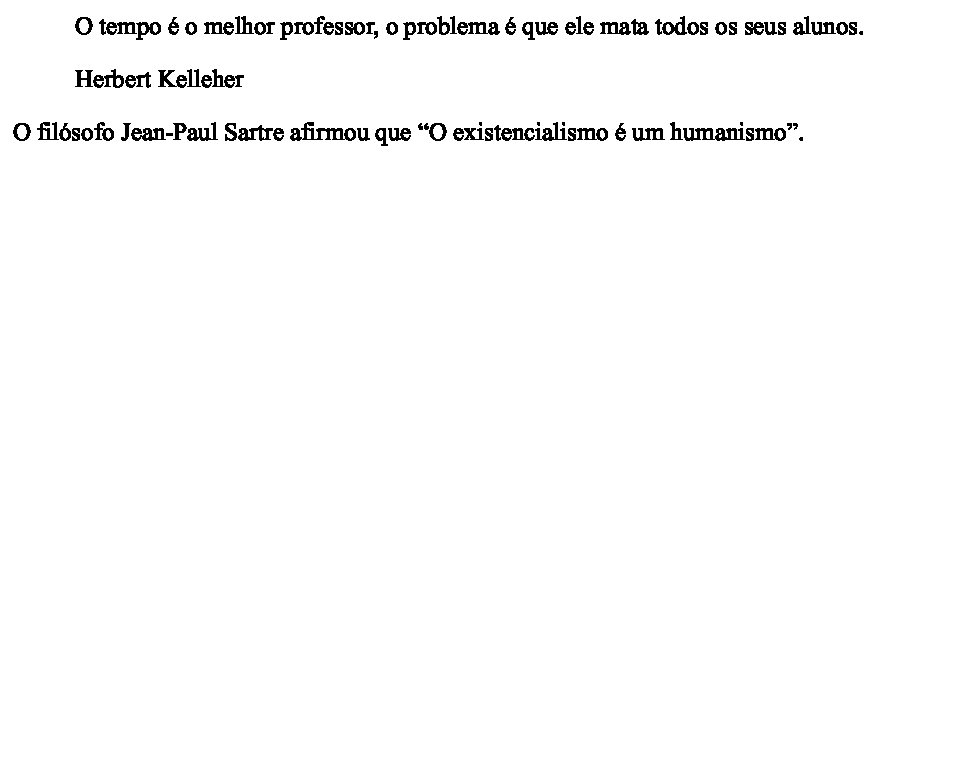
\includegraphics[width=1\textwidth, trim={0 10cm 0cm 0}]{Images/chapter03/html_citacoes.pdf}}
    \caption{Renderização dos códigos de citação desta seção.}
    \label{fig:html_citacoes}
\end{figure}

\section{Exercícios Propostos}

Essa série de exercícios envolve os conceitos abordados neste capítulo e também \textbf{pode demandar alguma pesquisa}. Reserve um tempo e um local adequados para fazer os exercícios sem distrações. Assim você absorverá muito mais o conteúdo estudado.

\begin{exercise}
Crie uma página HTML com seis títulos de diferentes níveis (1 a 6) e, abaixo de cada título, um parágrafo de texto com 50 palavras (use lorem ipsum).
\end{exercise}

\begin{exercise}
Adicione links ancorados em todos os parágrafos para voltarem ao título de nível 1.
\end{exercise}

\begin{exercise}
Adicione, ao fim, dentro de um parágrafo, um link externo apontando para a página da Wikipédia.
\end{exercise}

\begin{exercise}
Adicione, no início, dentro de um parágrafo, um link interno apontando para uma página chamada ``contato.html''.
\end{exercise}

\begin{exercise}
Crie um documento HTML que mostre o trecho de código-fonte apresentado no exemplo \ref{code_css_simples}, combinando os elementos \var{<pre>} e \var{<code>} para apresentar o código da melhor forma possível.
\end{exercise}

\begin{exercise}
Adicione destaques ao texto do documento HTML anterior usando elementos \textit{inline}, como \var{<strong>}, \var{<em>} e \var{<mark>}.
\end{exercise}

\begin{exercise}
Crie um documento HTML contendo um título de nível 1, dois parágrafos e uma citação longa.
\end{exercise}

\begin{exercise}
Adicione uma abreviação a um dos parágrafos do exercício anterior.
\end{exercise}

\begin{exercise}
Marque um trecho de um dos parágrafos do exercício anterior usando o elemento de marcação da HTML.
\end{exercise}

\begin{exercise}
Crie duas páginas HTML - index.html e contato.html - Com um título e um parágrafo cada. Ao fim da página index.html, adicione um link que navegue até a página contato.html e, ao fim de contato.html, adicione um link que volte para a página index.html. 
\end{exercise}

\section{Considerações Sobre o Capítulo}

Este capítulo apresentou os elementos textuais básicos da linguagem HTML, incluindo títulos, parágrafos, quebras de linha, blocos de citação, texto pré-formatado, texto de código-fonte e links. No capítulo seguinte, veremos como apresentar dados usando listas e tabelas.